\textbf{Texto para as questões 21 e 22}\par\medskip
\textbf{Computer-generated inclusivity: fashion turns to `diverse' AI models}\par
\textit{Fashion brands including Levi’s are having custom AI models created to `supplement' representation in size, skin tone and age}\par
Alaina Demopoulos — Mon 3 Apr 2023 11.00 BST\par\medskip
The star of Levi’s new campaign looks like any other model. Her tousled hair hangs over her shoulders as she gazes into the camera with that far-off high-fashion stare. But look closer, and something starts to seem a little off. The shadow between her chin and neck looks muddled, like a bad attempt at using Face Tune’s eraser effect to hide a double chin. Her French-manicured fingernails appear scrubbed clean and uniform in a creepy real doll kind of way.\par
The model is AI-generated, a digital rendering of a human being that will start appearing on Levi’s e-commerce website later this year. The brand teamed with LaLaLand.ai, a digital studio that makes customized AI models for fashion companies, to dream up this avatar.\par
Amy Gershkoff Bolles, Levi’s global head of digital and emerging technology strategy, announced the model’s debut at a Business of Fashion event in March. AI models \underline{will not} completely \underline{replace} the humans, she said, but will serve as a “supplement” intended to aid in the brand’s representation of various sizes, skin tones and ages.\par
“When we say supplement, we mean the AI-generated models can be used in conjunction with human models to potentially expand the number of models per product,” a Levi’s spokesperson said. “We are excited about a world where consumers can see more models on our site, potentially reflecting any combination of body type, age, size, race and ethnicity, enabling us to create a more personal and inclusive shopping experience.”\par
Michael Musandu, the founder of LaLaLand.ai, created the software in part because he struggled to find models who look like him. He \underline{was} born in Zimbabwe, raised in South Africa, and moved to the Netherlands to study computer science. “Any good technologist, instead of complaining about a problem, will build a future where you could actually have this representation,” Musandu said.\par
What about simply hiring a diverse cast of models? Musandu said that LaLaLand.ai is not meant to “replace” models, but allow brands to afford showing off different clothes on as many bodies as possible.\par
“It is not feasible for brands to shoot nine models for every single product they sell, because they’re not just hiring models, they’re hiring photographers, hair stylists and makeup artists for those models.” AI-generated images don’t need glam squads, so brands can cut costs they would spend on set by using fake avatars.\par
A spokesperson for Levi’s added: “The models Levi’s hires are already diverse and this will continue to be a priority for us. Over the past year, we’ve been focused on ensuring that those working on the content both in front and behind the camera are reflective of our broad consumer base.”\par
Yet the diversity that AI can provide \underline{is always going to be} virtual – a computer-generated sense of inclusivity. Are brands who generate, for example, black models for pieces where they only photographed a white human model engaging in a kind of digital blackface?\par
This is not a new question. There are already “digital influencers” like Lil Miquela and Shudu, fake avatars with millions of followers on social media. They \underline{model} Prada, Dior and Gucci clothing with the idea that their (human) audience will purchase the pieces. Neither model is white, but both have at least one white creator (Shudu was created by British fashion photographer Cameron-James Wilson and Miquela by Trevor McFedries and Sara Decou).\par
Criticism of Levi’s for casting AI models instead of real ones echoes the wave of response Lil Miquela got when she was first launched in 2016, or when Shudu made her debut two years later. The New Yorker’s Lauren Michele Jackson called Shudu “a white man’s digital projection of real Black womanhood”.\par
Unlike their mortal counterparts, these models also never age. Miquela, a “19-year-old Robot living in LA”, is forever 19 – making her a hot commodity in a youth-obsessed industry.\par
How long before these models are taking away jobs from real people? Sara Ziff, founder of the advocacy group The Model Alliance, is concerned, “capitalizing on someone else’s identity to the exclusion of hiring people who are actually Black could be compared to Blackface”, Ziff said.\par
Disponível em: https://www.theguardian.com/fashion/2023/apr/03/ai-virtual-models-fashion-brands. Acesso em: 3 ago. 2025. Adaptado.
\begin{figure}[htbp]
\centering
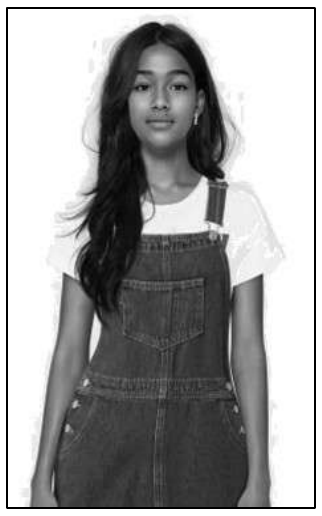
\includegraphics[width=0.42\linewidth]{static/simulados/coluni/figuras/2026/questao-20/figura-1.png}
\end{figure}

\textbf{COLUNI 2026 -- Questão 22}\par\medskip Leia as frases a seguir retiradas do texto:\par\medskip
I. AI models \underline{will not} completely \underline{replace} the humans.\par
II. He \underline{was} born in Zimbabwe.\par
III. Yet the diversity that AI can provide \underline{is always going to be} virtual.\par
IV. They \underline{model} Prada, Dior and Gucci clothing.\par\medskip
Os verbos e as expressões verbais destacados apresentam, respectivamente, a ideia de:\begin{enumerate}
\item futuro, passado, futuro e presente.
\item passado, presente, futuro e passado.
\item presente, futuro, presente e passado.
\item presente, passado, presente e presente.\end{enumerate}
